\documentclass[../main.tex]{subfiles}

\begin{document}

\subsection{Evolución de la Web.}
En esta sección se tratará de introducir y contextualizar las principales características que han definido a cada una de las etapas de la Web a lo largo del tiempo. Este análisis previo se centrará exclusivamente en la gestión del \textbf{almacenamiento de las credenciales} que identificarán a los usuarios, puesto que es el tema que nos atañe en este trabajo.
\\

\begin{figure}[htbp]
    \centering
    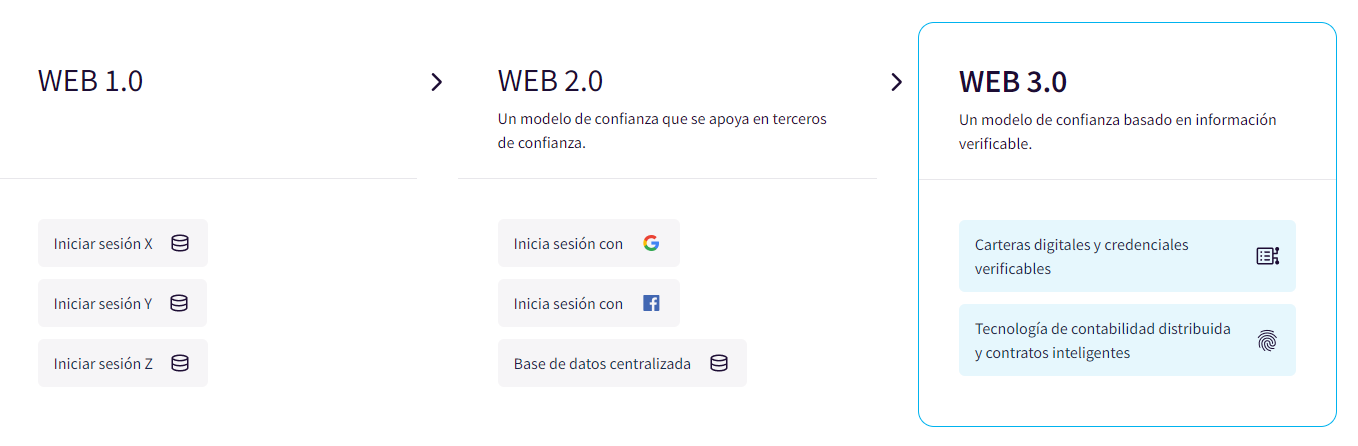
\includegraphics[width=1\linewidth]{images/EvolucionWeb.png}
    \caption{\textit{Gestión de las credenciales en cada etapa.} Fuente \cite{ebsiVCF}}
    \label{fig:evolucion}
\end{figure}

Durante su primera etapa, en la denominada como \textbf{Web 1.0} la autenticación no era una de las principales preocupaciones puesto que internet tenía fines informativos \cite{WebAuthentication}. Los usuarios accedían a los recursos web como si de un tablón de anuncios se tratase, por lo que la información debía ser de acceso libre y los sitios eran estáticos con apenas interactividad.

Sin embargo, los datos alojados en ella estaban siendo almacenados localmente en bases de datos distintas para cada servicio. Este hecho supuso un problema de \textbf{dispersión} y \textbf{duplicidad} de información a lo largo de la red que se vio enfatizado a medida que se introducían las primeras credenciales de usuario, guardándose además en \textbf{texto plano}.

Una vez se asentó la necesidad de identificar a los usuarios que accedían a los recursos web, dio comienzo la \textbf{Web 2.0} y con ella la introducción del dinamismo y el contenido generado por los propios usuarios. En lo referente a la seguridad, se optaron por algoritmos criptográficos \Gls{hash} para el almacenamiento de las credenciales y protocolos para el establecimiento seguro de la conexión como \Gls{HTTPS}, lo cual supuso una mejora sustancial a la anterior etapa.

No obstante, el problema de la dispersión y duplicidad de los datos seguía presente. De hecho, esto afectaba en gran medida al nuevo paradigma de las credenciales, puesto que nuevas soluciones basadas en la \textbf{confianza con terceros} ayudaron a la centralización de los datos.
\\

\begin{tcolorbox}[colback=gray!10!white, colframe=gray!50!black, title=Reflexión]\label{reflexion}
No es de extrañar que la segunda versión de la Web fuera una expansión de la primera que tratase de solventar los problemas originados por la misma, viéndose acentuados por la masiva adopción. Entonces, ¿ya hemos terminado? ¿Es lo mejor que podemos conseguir o existe algún aspecto con margen de mejora?
\end{tcolorbox}

\vspace{1cm} 

Actualmente nos encontramos en proceso de transición a la \textbf{Web 3.0} la cual promete traer un paradigma \textbf{descentralizado} (sin dependencia de terceras partes) aún manteniendo las bases construidas en las anteriores etapas. Para ello propone introducir nuevas tecnologías como las Carteras de Identidad Digital, el \acrfull{DID} y la \acrfull{VC} que mejorarán la seguridad y privacidad de los usuarios, a la vez que permitirá a las personas recuperar el control sobre sus propios datos personales \cite{WebAuthentication}.

\newpage
\subsection{Identidad Autosoberana.}\label{Identidad Autosoberana}
\subfile{IdentidadAutosoberana}

\newpage
\subsection{Identidad Digital Europea.}\label{Identidad Digital Europea}
\subfile{IdentidadDigitalEuropea}

\end{document}
